\section{Pipelines and Networks}
Pipe networks, like single path pipelines, are analyzed for head losses in order to size pumps, determine demand management strategies, and ensure minimum pressures in the system.   Conceptually the same principles are used for steady flow systems: conservation of mass and energy; with momentum used to determine head losses.

\subsection{Pipe Networks -- Topology}
Network topology refers to the layout and connections.  
Networks are built of nodes (junctions) and arcs (links).  
\subsubsection{Continunity (at a node)}

Water is considered incompressible in steady flow in pipelines and pipe networks, and the
conservation of mass reduces to the volumetric 
flow rate, $Q$,
\begin{equation}
Q = AV 
\end{equation}

where $A$ is the cross sectional of the pipe, and $V$ is the mean section velocity. Typical units
for discharge is liters per second (lps), gallons per minute (gpm), cubic meters per second
(cms), cubic feet per second (cfs), and million gallons per day (mgd). 
The continuity equation in two cross-sections of a pipe as depicted in Figure \ref{fig:continuity-across-sections} is

\begin{equation}
A_1V_1 = A_2V_2
\end{equation}

Junctions (nodes) are where two or more pipes join together. 
A three-pipe junction node with constant external demand is shown in Figure 10. The continuity equation for the
junction node is
\begin{equation}
Q_1 - Q_2 - Q_3 - D = 0
\end{equation}

\begin{figure}[h!] %  figure placement: here, top, bottom, or page
   \centering
   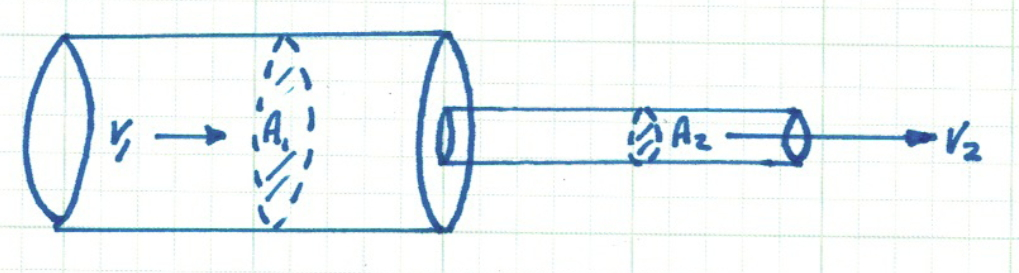
\includegraphics[width=5in]{./8-PipeNetworkHydraulics/continuity-across-sections.jpg} 
   \caption{Continuity of mass (discharge) across a change in cross section}
   \label{fig:continuity-across-sections}
\end{figure}

\begin{figure}[h!] %  figure placement: here, top, bottom, or page
   \centering
   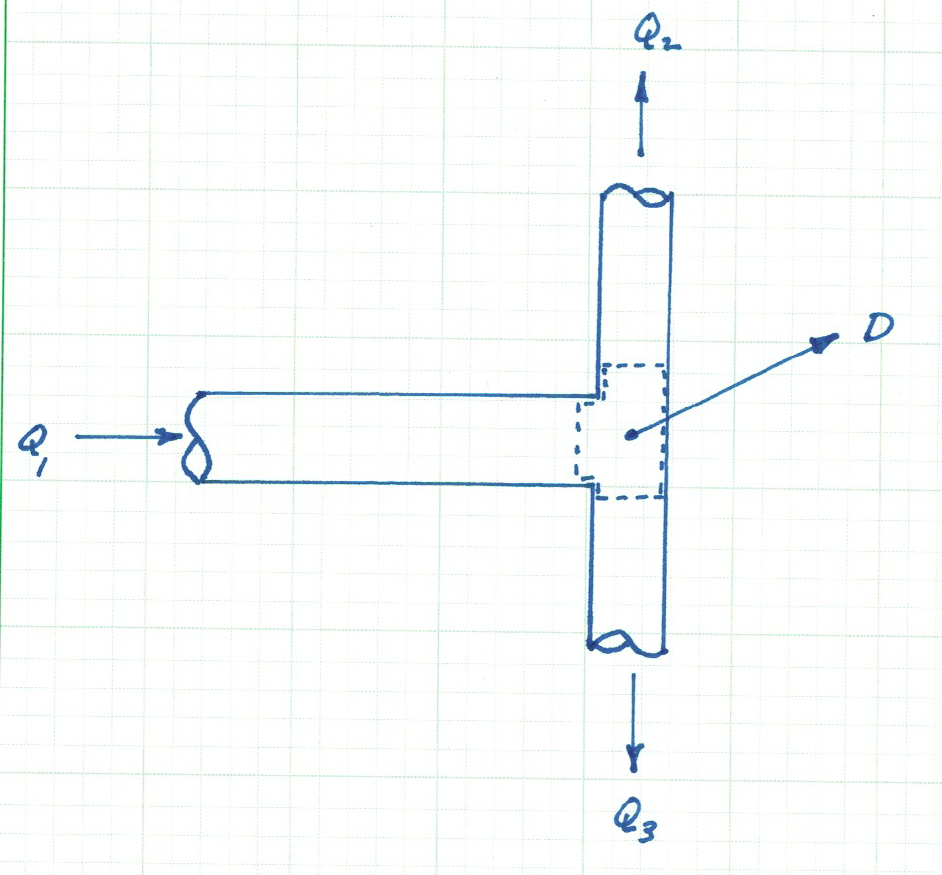
\includegraphics[width=5in]{./8-PipeNetworkHydraulics/continuity-at-node.jpg} 
   \caption{Continuity of mass (discharge) across a node (junction)}
   \label{fig:continuity-at-node}
\end{figure}

In design analysis, all demands on the system are located at junctions (nodes), and the flow connecting junctions is assumed to be uniform across the cross sections (so that mean velocities apply). 
If a substantial demand is located between nodes, then an additional node is established at the demand location. 

\subsubsection{Energy Loss (along a link)}
Equation \ref{eqn:closed-conduit-energy-equation} is the one-dimensional steady flow form of the energy equation typically applied for pressurized conduit hydraulics.
 
\begin{equation}
\frac{p_1}{\rho g}+\alpha_1 \frac{V_1^2}{2g} + z_1 + h_p =
\frac{p_2}{\rho g}+\alpha_2 \frac{V_2^2}{2g} + z_2 + h_t + h_l
\label{eqn:closed-conduit-energy-equation}
\end{equation}

where $\frac{p}{\rho g}$ is the pressure head at a location, $\alpha \frac{V^2}{2g}$ is the velocity head at a location, $z$ is the elevation, $h_p$ is the added head from a pump, $h_t$ is the added head extracted by a turbine, and $h_l$ is the head loss between sections 1 and 2.   Figure \ref{fig:closed-conduit-energy} is a sketch that illustrates the various components in Equation \ref{eqn:closed-conduit-energy-equation}.

\begin{figure}[h!] %  figure placement: here, top, bottom, or page
   \centering
   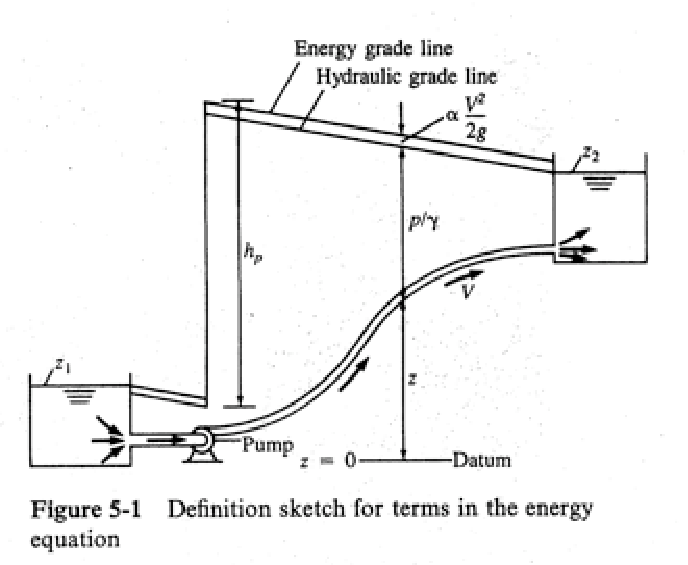
\includegraphics[width=4in]{./8-PipeNetworkHydraulics/closed-conduit-energy.pdf} 
   \caption{Definition sketch for energy equation}
   \label{fig:closed-conduit-energy}
\end{figure}

In network analysis this energy equation is applied to a link that joins two nodes.
Pumps and turbines would be treated as separate components (links) and their hydraulic behavior must be supplied using their respective pump/turbine curves.

\subsubsection{Velocity Head}
The velocity in $\alpha \frac{V^2}{2g}$ is the mean section velocity and is the ratio of discharge to flow area.  The kinetic energy correction coefficient is 
\begin{equation}
\alpha=\frac{\int_A u^3 dA}{V^3 A}
\label{eqn:kinetic-energy-correction}
\end{equation}
where $u$ is the point velocity in the cross section (usually measured relative to the centerline or the pipe wall; axial symmetry is assumed).   Generally values of $\alpha$ are 2.0 if the flow is laminar, and approach unity (1.0) for turbulent flow.  In most water distribution systems the flow is usually turbulent so $\alpha$ is assumed to be unity and the velocity head is simply $\frac{V^2}{2g}$.

\subsubsection{Added Head --- Pumps}
The head supplied by a pump is related to the mechanical power supplied to the flow.   Equation \ref{eqn:pump-power} is the relationship of mechanical power to added pump head.
\begin{equation}
\eta P=Q\rho g h_p
\label{eqn:pump-power}
\end{equation}
where the power supplied to the motor is $P$ and the  ``wire-to-water'' efficiency is $\eta$.

If the relationship is re-written in terms of added head\footnote{A negative head loss!} the pump curve is 
\begin{equation}
h_p = \frac{\eta P}{Q\rho g}
\label{eqn:pump-curve}
\end{equation}

This relationship illustrates that as discharge increases (for a fixed power) the added head decreases.
Power scales at about the cube of discharge, so pump curves for computational application typically have a mathematical structure like
\begin{equation}
h_p =  H_{\text{shutoff}} - K_{\text{pump}}Q^{\text{exponent}}
\label{eqn:pump-curve-2}
\end{equation}

\subsubsection{Extracted Head --- Turbines}
The head recovered by a turbine is also an ``added head'' but appears on the loss side of the equation.   Equation \ref{eqn:turbine-power} is the power that can be recovered by a turbine (again using the concept of ``water-to-wire'' efficiency is 
\begin{equation}
P=\eta Q\rho g h_t
\label{eqn:turbine-power}
\end{equation}


\subsection{Pipe Head Loss Models}
The Darcy-Weisbach, Chezy, Manning, and Hazen-Williams formulas are relationships between physical pipe characteristics, flow parameters, and head loss.   The Darcy-Weisbach formula is the most consistent with the energy equation formulation  being derivable (in structural form) from elementary principles.
\begin{equation}
h_{L_f}=f \frac{L}{D} \frac{V^2}{2g}
\label{eqn:dw-headloss}
\end{equation}
where $h_{L_f}$ is the head loss from pipe friction, $f$ is a dimensionless friction factor, $L$ is the pipe length, $D$ is the pipe characteristic diameter, $V$ is the mean section velocity, and $g$ is the gravitational acceleration.  

The friction factor, $f$, is a function of Reynolds number $Re_D$ and the roughness ratio $\frac{k_s}{D}$.
\begin{equation}
f=\sigma(Re_D,\frac{k_s}{D})
\label{eqn:friction-factor-dimensionless}
\end{equation}

The structure of $\sigma$ is determined experimentally.  Over the last century the structure is generally accepted to be one of the following depending on flow conditions and pipe properties
\begin{enumerate}
\item Laminar flow (Eqn 2.36, pg. 17~\cite{chin2006}) :  
\begin{equation}
f=\frac{64}{Re_D}
\label{eqn:friction-factor-laminar}
\end{equation}
\item Hydraulically Smooth Pipes(Eqn 2.34 pg. 16~\cite{chin2006}):
\begin{equation}
\frac{1}{\sqrt{f}}=-2 log_{10} (\frac{2.51}{Re_d \sqrt{f} })
\label{eqn:friction-factor-smooth}
\end{equation}
\item Hydraulically Rough Pipes(Eqn 2.34 pg. 16~\cite{chin2006}):
\begin{equation}
\frac{1}{\sqrt{f}}=-2 log_{10} (\frac{\frac{k_e}{D}} {3.7})
\label{eqn:friction-factor-rough}
\end{equation}
\item Transitional Pipes (Colebrook-White Formula)(Eqn 2.35 pg. 17~\cite{chin2006}):
\begin{equation}
\frac{1}{\sqrt{f}}=-2 log_{10} (\frac{\frac{k_e}{D}} {3.7} + \frac{2.51}{Re_d \sqrt{f} } )
\label{eqn:friction-factor-CW}
\end{equation}
\item Transitional Pipes (Jain Formula)(Eqn 2.39 pg. 19~\cite{chin2006}):
\begin{equation}
f=\frac{0.25}{[log_{10} (\frac{\frac{k_e}{D}} {3.7} + \frac{5.74}{Re_d^{0.9} } )]  ^2}
\label{eqn:friction-factor-Jain}
\end{equation}
\end{enumerate} 




\subsection{Illustrative Example}




\subsubsection{Check geometry}
A unique solution exists only if the sum of the node count and loop count is equal to the pipe count.  In the current example this sum is 11, but the drawing shows only 10 pipes.  A modeling trick is to add a fictitious pipe at either a supply of demand point to satisfy this geometric requirement.  The particulars of this imaginary pipe are irrelevant as flow in this pipe should vanish at the solution.


\subsubsection{Prepare $f,K,Re$ Tables}
The next step is to prepare tables for use in the head loss equations.  In these notes, the Darcy-Weisbach formula is used for head loss, thus the relevant equations for any particular pipe are:
\begin{enumerate}
\item The head loss coefficient (just the constant part) to be multiplied by $|Q|Q$ to obtain loss for the pipe;
\begin{equation}
K=\frac{4 \rho}{\pi^2 g D^5}
\end{equation}

\item The Reynolds number coefficient, to be multiplied by $Q$ to obtain the pipe Reynolds number for determination of friction factors.


\begin{equation}
\frac{Re}{Q}=\frac{8L}{\mu \pi D}
\end{equation}
\item An the friction factor table (if variable factors are to be used); typically the Colebrook-White formula is used, but table look-up is also valid and fast.  In this example fixed values will be used, so the Reynolds number component is superfluous.

\end{enumerate}

The head loss in any pipe is $H_{loss} = f K |Q| Q$

\subsubsection{Write the mass balance for each node and head loss for each loop}
This step builds the equation system, the matrix below has two partitions, the upper partition corresponds to the nodal equations, and the lower partition to the loop equations.  Notice that the lower partition will change value for any change in the discharges.

\setcounter{MaxMatrixCols}{15}
%\begin{equation}
%\begin{matrix}
%-1& 0 & 0  & 0 & 0 & -1& 0 & 0 & 0 &0 & 0 & Q_1& = & -10\\
% 1& -1& 0  & -1 & 0 & 0& 0 & 0 & 0 &0 & 0 & Q_2& = & 0\\
% 0& 1 & -1 & 0 & 0 & 0& 0 & 0 & 0 &0 & 0 & Q_3& = & 0\\
% 0& 0 & 0  & 0 & 1 & 1& -1 & 0 & 0 &0 & 0 & Q_4& = & 0\\
%0& 0& 0 & 1 & -1 & 0 & 0 & 0 & -1 &0 & 0 & Q_5& = & 0\\
%0& 0& 0 & 0 & 0 & 0& 1 & -1 & 0 &0 & 0 & Q_6& = & 0\\
%0& 0& 0 & 0 & 0 & 0& 0 & 1 & 1 &1 & 0 & Q_7& = &0\\
%0& 0& 1 & 0 & 0 & 0& 0 & 0 & 0 &-1 & -1 & Q_8& = & 10\\
%fK|Q_1|& 0& 0 & fK|Q_4| & fK|Q-5| & - fK|Q_6|& 0 & 0 & 0 &0 & 0 & Q_9& = & 0\\
%0& fK|Q_2|& fK|Q_3| & -fK|Q_4| & 0 & 0& 0 & 0 & -fK|Q_9| &fK|Q_10| & 0 & Q_{10}& = & 0\\
%0& 0& 0 & 0 & -fK|Q_5| & 0& -fK|Q_7| & -fK|Q_8| & fK|Q_10| &0 & 0 & Q_{11}& = & 0\\
% \end{matrix}
% \end{equation}

\begin{displaymath}
\footnotesize
\begin{matrix}
-1& 0 & 0  & 0 & 0 & -1& 0 & 0 & 0 &0 & 0  \\
 1& -1& 0  & -1 & 0 & 0& 0 & 0 & 0 &0 & 0  \\
 0& 1 & -1 & 0 & 0 & 0& 0 & 0 & 0 &0 & 0  \\
 0& 0 & 0  & 0 & 1 & 1& -1 & 0 & 0 &0 & 0 \\
0& 0& 0 & 1 & -1 & 0 & 0 & 0 & -1 &0 & 0 \\
0& 0& 0 & 0 & 0 & 0& 1 & -1 & 0 &0 & 0 \\
0& 0& 0 & 0 & 0 & 0& 0 & 1 & 1 &1 & 0 \\
0& 0& 1 & 0 & 0 & 0& 0 & 0 & 0 &-1 & -1 \\
fK|Q_1|& 0& 0 & fK|Q_4| & fK|Q_5| & - fK|Q_6|& 0 & 0 & 0 &0 & 0 \\
0& fK|Q_2|& fK|Q_3| & -fK|Q_4| & 0 & 0& 0 & 0 & -fK|Q_9| &fK|Q_{10}| & 0 \\
0& 0& 0 & 0 & -fK|Q_5| & 0& -fK|Q_7| & -fK|Q_8| & fK|Q_{10}| &0 & 0 \\
 \end{matrix}
 \normalsize
 \end{displaymath}
 
 The convention used here is that flow into a node is algebraically positive, while flow away from a node is negative.  The sign convention in the loop partition is that if the loop traverse is the same direction as the assumed flow, then the sign convention is a positive loss, while a negative loss is computed for the opposite situation.  The array above is a coefficient matrix dependent on discharge.  This array is represented here as $\mathbf{A}(\mathbf{Q})$. 
 
 The discharges are written as the vector  $\mathbf{Q}$
 
 \begin{displaymath}
\footnotesize
\begin{matrix}
Q_1 \\
Q_2  \\
Q_3 \\
Q_4 \\
Q_5 \\
Q_6 \\
Q_7\\
Q_8 \\
Q_9 \\
Q_{10} \\
Q_{11} \\
 \end{matrix}
 = \mathbf{Q}
 \normalsize
 \end{displaymath}
 
 The demand is written as the vector $\mathbf{D}$
 \begin{displaymath}
\footnotesize
\begin{matrix}
-10 \\
0  \\
0 \\
0\\
0 \\
0 \\
0\\
10 \\
0 \\
0 \\
0 \\
 \end{matrix}
 = \mathbf{D}
 \normalsize
 \end{displaymath} 
 
So the resulting system of equations\footnote{Non-linear because of the $|Q|Q$ term.} are 

 \begin{equation}
[\mathbf{A}(\mathbf{Q})] \cdot \mathbf{Q} = \mathbf{D}
\end{equation}

\subsection{Finding a Solution to the Network Equations}
The network equations include the node equations\footnote{These equations are statements of conservation of mass.} and the loop equations\footnote{These equations are statements of conservation of energy and independence of path.}.  The set of equations are solved simultaneously for pipe discharge, and then these results are used to determine system pressures or other nodal quantities.  The system for a pipeline network happens to be a quadratic system of equations, therefore non-linear, and therefore some adaptation of linear solvers is used.

At the ``correct'' solution the following matrix-vector system is true.

\begin{equation}
[\mathbf{A}(\mathbf{Q})] \cdot \mathbf{Q} = \mathbf{D}
\end{equation}

In this expression, $\mathbf{A}$ is a function of $\mathbf{Q}$; therefore the coefficient matrix is a function of the solution vector --- a non-linear system.  If the system were a univariate non-linear equation, we would proceed by subtracting the right-hand side from the left hand side and re-expressing the entire relationship as a function of the solution variable that is supposed to equal $0$.

\subsection{Newton-Raphson Method Theory}
The Newton-Raphson method extends the classical Newton's method to vector valued functions of vector arguments.  The first derivative of Newton;s method is replaced by the Jacobian of the function, but otherwise the method is for all purposes identical to the univariate Newton's method.

Starting with the network equations, they are rewritten into a functional form suitable for a Newton's-type approach.
\begin{equation}
[\mathbf{A}(\mathbf{Q})] \cdot \mathbf{Q} - \mathbf{D} = \mathbf{f}(\mathbf{Q}) = \mathbf{0}
\end{equation}

Recall from Newton's method that

\begin{equation}
x_{k+1}=x_{k} - (\frac{df}{dx}\mid_{x_k})^{-1} f(x_k)
\end{equation}

thus the extension to the pipeline case is

\begin{equation}
\mathbf{Q}_{k+1}=\mathbf{Q}_{k} - [\mathbf{J}(\mathbf{Q}_{k})]^{-1} \mathbf{f}(\mathbf{Q}_k) 
\end{equation}

where
$\mathbf{J}(\mathbf{Q}_{k})$ is the Jacobian of the coefficient matrix $\mathbf{A}$ evaluated at $\mathbf{Q}_{k}$.   Although a bit cluttered, here is the formula for a single update step, with the matrix, demand vector, and the solution vector in their proper places.

\begin{equation}
\mathbf{Q}_{k+1}=\mathbf{Q}_{k} - [\mathbf{J}(\mathbf{Q}_{k})]^{-1} \{[\mathbf{A}(\mathbf{Q}_k)] \cdot \mathbf{Q}_k - \mathbf{D}\}
\end{equation}

The Jacobian of the pipeline model is a matrix with the following properties:
\begin{enumerate}
\item The partition of the matrix that corresponds to the node formulas is identical to the original coefficient matrix --- it will be comprised of $0~\text{or}~\pm~1$ in the same pattern at the equivalent partition of the $\mathbf{A}$ matrix.
\item The partition of the matrix that corresponds to the loop formulas, will consist of values that are twice the values of the coefficients in the original coefficient matrix (at any supplied value of $\mathbf{Q}_k$.
\end{enumerate}

In the current example the Jacobian would look like the following array (columns and rows are abbreviated to fit the page) :

\begin{displaymath}
\footnotesize
\begin{matrix}
-1& 0 & 0  & \dots &0 & 0  \\
 1& -1& 0  & \dots &0 & 0  \\
 \dots \\
\dots \\
0& 0& 1 & \dots  &-1 & -1 \\
2fK|Q_1|& 0& 0 & \dots &0 & 0 \\
0&2 fK|Q_2|& 2fK|Q_3|  & \dots &2fK|Q_{10}| & 0 \\
0& 0& 0 & \dots &0 & 0 \\
 \end{matrix}
 \normalsize
 \end{displaymath}

In this document, the pipeline solution is a true ``Newton's'' method because analytical Jacobian values are used.  If a numerical method to approximate the derivatives is used it would be called a quasi-Newton method.

As an algorithm, the engineer would supply a guess for $\mathbf{Q}_k$, compute the update value, used this just computed value as the new guess, and repeat the computation until the computed vector is relatively unchanging.  Typically, even with a poor first guess (but convergent), the solution can be found in $\approx~2~\times~\text{rank}(\mathbf{A})$

This method is the basis of nearly all network models (it is even used in groundwater hydraulics and surface water networks).  The method with some effort can be extended to transient systems\footnote{In a transient solver, there would be a set of iterations per time-step, hence the method is used over-and-over to evolve forward in time.  In a transient case, analytical derivatives would be extremely desirable, but if geometry changes as in open channel cases, the programs usually sacrifice speed and use numerical approximation of the Jacobian at each time step.}.

\subsection{Pipe Networks -- Computing Flow Distributions}

This subsection presents a network simulator program in \textbf{R} using a simple example to motivate the script. 

 
\begin{lstlisting}[caption=R code demonstrating a Pipeline Network Simulator \\ This fragment of code reads the data file and converts the lines (read as text) into numeric values for subsequent processing, label=lst:PipeNetwork1]
# Pipe Network Simulator Using Newton-Raphson
########################################################
########## Read the Input Data from a file #############
########################################################
zz <- file("PipeNetwork.txt", "r") # Open a connection named zz to file named PipeNetork.txt
nodes <- as.numeric(readLines(zz, n = 1, ok = TRUE, warn = TRUE,encoding = "unknown", skipNul = FALSE))
pipes <-as.numeric(readLines(zz, n = 1, ok = TRUE, warn = TRUE,encoding = "unknown", skipNul = FALSE))
loops <-as.numeric(readLines(zz, n = 1, ok = TRUE, warn = TRUE,encoding = "unknown", skipNul = FALSE))
diameter <- (readLines(zz, n = 1, ok = TRUE, warn = TRUE,encoding = "unknown", skipNul = FALSE))
distance <- (readLines(zz, n = 1, ok = TRUE, warn = TRUE,encoding = "unknown", skipNul = FALSE))
roughness <- (readLines(zz, n = 1, ok = TRUE, warn = TRUE,encoding = "unknown", skipNul = FALSE))
viscosity <- (readLines(zz, n = 1, ok = TRUE, warn = TRUE,encoding = "unknown", skipNul = FALSE))
flowguess <- (readLines(zz, n = 1, ok = TRUE, warn = TRUE,encoding = "unknown", skipNul = FALSE))
nodearcs <- (readLines(zz, n = nodes, ok = TRUE, warn = TRUE,encoding = "unknown", skipNul = FALSE))
looparcs <- (readLines(zz, n = loops, ok = TRUE, warn = TRUE,encoding = "unknown", skipNul = FALSE))
rhs_true <- (readLines(zz, n = loops, ok = TRUE, warn = TRUE,encoding = "unknown", skipNul = FALSE))
close(zz)
#############################################################
######## convert the multiple column strings into numeric  #############
#############################################################
diameter <-as.numeric(unlist(strsplit(diameter,split=" ")))
distance <-as.numeric(unlist(strsplit(distance,split=" ")))
roughness <-as.numeric(unlist(strsplit(roughness,split=" ")))
viscosity <-as.numeric(unlist(strsplit(viscosity,split=" ")))
flowguess <-as.numeric(unlist(strsplit(flowguess,split=" ")))
nodearcs <-as.numeric(unlist(strsplit(nodearcs,split=" ")))
looparcs <-as.numeric(unlist(strsplit(looparcs,split=" ")))
rhs_true <-as.numeric(unlist(strsplit(rhs_true,split=" ")))
#############################################################
######### convert nodearcs and looparcs into matrices    ##############
#############################################################
nodearcs <-matrix(nodearcs,nrow=nodes,ncol=pipes,byrow = TRUE)
looparcs <-matrix(looparcs,nrow=loops,ncol=pipes,byrow = TRUE)
#############################################################
#### Some constants, probably should make into inputs ################
#############################################################
HowMany <- 25
tolerance1 <- 1e-24
tolerance2 <- 1e-16
#############################################################
################## need some storage vectors ####################
#############################################################
velocity_pipe <-numeric(0)
reynolds <- numeric(0)
friction <- numeric(0)
geometry <- numeric(0)
lossfactor <- numeric(0)
funcMatrix <- matrix(0,nodes+loops,pipes)
jacbMatrix <- matrix(0,nodes+loops,pipes)
gq <- numeric(0)
\end{lstlisting}   

Listing \ref{lst:PipeNetwork2} is a listing that contains the various support functions used, including a function to compute friction factors, reynolds number, and some geometric factors that are used to simulate the pipeline network.
\clearpage

\begin{lstlisting}[caption=R code demonstrating a Pipeline Network Simulator \\ This fragment of code contains the functions for computing head losses, label=lst:PipeNetwork2]
#############################################################
##############  Forward Define Support Functions   #################
#############################################################
# Jain Friction Factor Function -- Tested OK 23SEP16
friction_factor <- function(roughness,diameter,reynolds){
  temp1 <- roughness/(3.7*diameter);
  temp2 <- 5.74/(reynolds^(0.9));
  temp3 <- log10(temp1+temp2);
  temp3 <- temp3^2;
  friction_factor <- 0.25/temp3;
  return(friction_factor)
}
# Velocity Function
velocity <- function(diameter,discharge){
  velocity <- discharge/(0.25*pi*diameter^2)
  return(velocity)
}
# Reynolds Number Function
reynolds_number <- function(velocity,diameter,mu){
  reynolds_number <- abs(velocity)*diameter/mu
  return(reynolds_number)
}
# Geometric factor function
k_factor <- function(howlong,diameter,gravity){
  k_factor <- (16*howlong)/(2.0*gravity*pi^2*diameter^5)
  return(k_factor)
}
\end{lstlisting}   

Listing \ref{lst:PipeNetwork3} is a listing that contains the computations implemented each iteration to compute the loss functions and populate the \textbf{A} matrix that multiplies the $Q^{k}$ vector to produce the model right-hand side.

\begin{lstlisting}[caption=R code demonstrating a Pipeline Network Simulator \\ This fragment of code contains the computations that are used to build the coefficients in the \textbf{Ax=B} system, label=lst:PipeNetwork3]
###############################################################
# compute geometry factors (only need once, goes outside iteration loop)
for (i in 1:pipes)
{
  geometry[i] <- k_factor(distance[i],diameter[i],32.2)
}
###############################################################
############# iteration outer loop start here #################
###############################################################
for (iteration in 1:HowMany){
# compute current velocity
for (i in 1:pipes)
{
  velocity_pipe[i]<-velocity(diameter[i],flowguess[i])
}
# compute current reynolds
for (i in 1:pipes) 
{
  reynolds[i]<-reynolds_number(velocity_pipe[i],diameter[i],viscosity)
}
# compute current friction factors
for (i in 1:pipes) 
{
  friction[i]<-friction_factor(roughness[i],diameter[i],reynolds[i])
}
# compute current loss factor
for (i in 1:pipes)
{
  lossfactor[i] <- friction[i]*geometry[i]*abs(flowguess[i])  
}
# build the function matrix
for (i in 1:nodes)
{
  for (j in 1:pipes)
  {
    funcMatrix[i,j] <- nodearcs[i,j]
  }
}
for (i in nodes+1:loops)
{
  for(j in 1:pipes)
  {
    funcMatrix[i,j] <- looparcs[i-nodes,j]*lossfactor[j]
  }
}
\end{lstlisting}   

Listing \ref{lst:PipeNetwork4} is a listing that contains the computations implemented each iteration to compute the Jacobian matrix that is used to compute the update.  The fragment also contains the stopping criteria and the write to \texttt{stdio()} to report the results to the programmer.

\begin{lstlisting}[caption=R code demonstrating a Pipeline Network Simulator \\ This fragment of code contains the computations that are used to build the Jacobian matrix, label=lst:PipeNetwork4]
# build the current jacobian matrix
for (i in 1:nodes)
{
  for (j in 1:pipes)
  {
    jacbMatrix[i,j] <- nodearcs[i,j]
  }
}
for (i in nodes+1:loops)
{
  for(j in 1:pipes)
  {
    jacbMatrix[i,j] <- looparcs[i-nodes,j]*2*lossfactor[j]
  }
}
jacbMatrix
# now try the multiplication to build the G(Q) vector
gq <- funcMatrix %*% flowguess - rhs_true # cool -- working to here as expected
# now the tricky part! want to solve the linear system Jacob*dQ = G(Q) for dQ -- system is linear
dq <- solve(jacbMatrix,gq)
# now update the flows
flownew <- flowguess - dq
# now test for stopping
test <- abs(flownew - flowguess)
if(t(test) %*% test < tolerance1)
{
  message("Update not changing -- exit loop and report current update")
  message("Iteration count = ",iteration)
  flowguess <- flownew
  break
}
test <- abs(gq)
if(t(test) %*% test < tolerance2)
{
  message("G(Q) close to zero -- exit loop and report current update")
  message("Iteration count = ",iteration)
  flowguess <- flownew
  break
}
flowguess <- flownew
}
###############################################################
########### End of iteration loop -- solution below ###########
###############################################################
message("Current results ")
print(cbind(flowguess, gq, dq))
\end{lstlisting}   



\subsection{Pipe Networks Solution Methods}
Several methods are used to produce solutions (estimates of discharge, head loss, and pressure) in a network.  
An early one, that only involves analysis of loops is the Hardy-Cross method.  
A later one, more efficient, is a Newton-Raphson method that uses node equations to balance discharges and demands, and loop equations to balance head losses.  
However, a rather ingenious method exists developed by \cite{Haman1971}, where the flow distribution and head values are determined simultaneously.   The task here is to implement the \cite{Haman1971} method on the problem below -- first some necessary definitions and analysis.

\subsection{Network Analysis}
\begin{figure}[h!] %  figure placement: here, top, bottom, or page
   \centering
   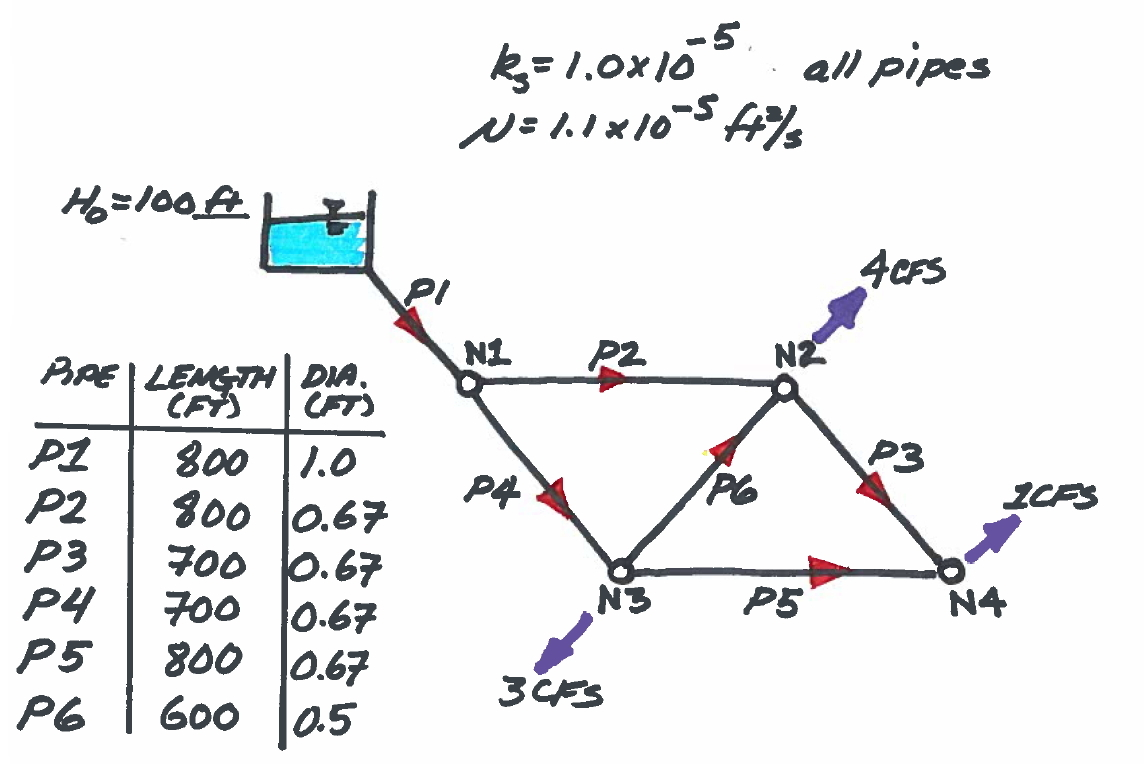
\includegraphics[width=5in]{./8-PipeNetworkHydraulics/pipe-net-hybrid.jpg} 
   \caption{Pipe network for illustrative example with supply and demands identified.  Pipe dimensions and diameters are also depicted.}
   \label{fig:pipe-net-hybrid}
\end{figure}

Figure \ref{fig:pipe-net-hybrid} is a sketch of the problem that will be used.  The network supply is the fixed-grade node in the upper left hand corner of the drawing.  The remaining nodes (N1 -- N4) have demands specified as the purple outflow arrows.
The pipes are labeled (P1 -- P6), and the red arrows indicate a positive flow direction, that is, if the flow is in the indicated direction, the numerical value of flow (or velocity) in that link would be a positive number.

Define the flows in each pipe and the total head at each node as $Q_i$ and $H_i$ where the subscript indicates the particular component identification.  Expressed as a vector, these unknowns are:
\setcounter{MaxMatrixCols}{15}
\begin{displaymath}
\begin{matrix}
[Q_1, & Q_2, & Q_3,  & Q_4, & Q_5, & Q_6, & H_1, & H_2, & H_3, &H_4 ]& =  & \textbf{x} \\
 \end{matrix}
 \end{displaymath}

If we analyze continuity for each node we will have 4 equations (corresponding to each node) for continunity, for instance for Node N2 the equation is 

\begin{displaymath}
\begin{matrix}
~& Q_2 & -Q_3  & ~ & ~ & Q_6 & ~ & ~ & ~ &~ & =  & 4\\
 \end{matrix}
 \end{displaymath}
 
Similarily if we define head loss in any pipe as $\Delta H_i = f \frac{8 L_i}{\pi^2 g D_i^5} |Q_i| Q_i$ or $\Delta H_i = L_i Q_i$, where $L_i = f \frac{8 L_i}{\pi^2 g D_i^5} |Q_i|$, then we have 6 equations (corresponding to each pipe) for energy, for instance for Pipe (P2) the equation is\footnote{The seemingly awkward way of writing the equations will become apparent shortly!}

\begin{displaymath}
\begin{matrix}
~& -L_2Q_2& ~ & ~ & ~ & ~& H_1 & -H_2 & ~ & ~ & = & 0\\
 \end{matrix}
 \end{displaymath}
 
 If we now write all the node equations then all the pipe equations we could construct the following coefficient matrix below:\footnote{The horizontal lines divide the node and the pipe equations.  The upper partition are the node equations in Q and H, the lower partition are the pipe equations in Q and H}
 
\begin{displaymath}
\begin{matrix}
%Q_1 & Q_2 & Q_3  & Q_4 & Q_5 & Q_6 & H_1 & H_2 & H_3 &H_4 & ~  & ~ \\
\hline
~1&-1 & 0  & -1 & 0 & 0 & 0 & 0 & 0 &0 \\
0&~1 & -1  & 0 & 0 &~1 & 0 & 0 & 0 &0 \\
0& 0 & 0 &~1 & -1 & -1 & 0 & 0 & 0 &0 \\
0& 0 &~1  & 0 &~1 & 0 & 0  & 0 & 0 &0 \\
\hline
-L_1& 0& 0 & 0 & 0 & 0 & -1 & 0 & 0 &0 \\
0& -L_2& 0 & 0 & 0 & 0&~1 & -1 & 0 &0 \\
0& 0& -L_3 & 0 & 0 & 0& 0 &~1 & 0 & -1 \\
0& 0& 0 & -L_4 & 0 & 0&~1 & 0 & -1 & 0 \\
0& 0& 0 & 0 & -L_5 & 0& 0 & 0 &~1 & -1 \\
0& 0& 0 &0 & 0 & -L_6& 0 & -1 &~1 & 0 \\
\hline
 \end{matrix}
 \end{displaymath}
 
Declare the name of this matrix $\textbf{A(x)}$, where $\textbf{x}$ denotes the unknown vector of Q augmented by H as above.  Next consider the right-hand-side at the correct solution (as of yet still unknown!) as

\begin{displaymath}
\begin{matrix}
[0, & 4, & 3,  & 1, & -100 , & 0, & 0, & 0, & 0, &0 ] = \textbf{b}\\
 \end{matrix}
 \end{displaymath}

So if the coefficient matrix is correct then the following system would result:
\begin{displaymath}
\mathbf{A(x)} \cdot \mathbf{x} = \mathbf{b}
  \end{displaymath}
  
  which would look like
  
 \begin{gather}
\begin{pmatrix}
~1&-1 & 0  & -1 & 0 & 0 & 0 & 0 & 0 &0 \\
0&~1 & -1  & 0 & 0 &~1 & 0 & 0 & 0 &0 \\
0& 0 & 0 &~1 & -1 & -1 & 0 & 0 & 0 &0 \\
0& 0 &~1  & 0 &~1 & 0 & 0  & 0 & 0 &0 \\
\hline
-L_1& 0& 0 & 0 & 0 & 0 & -1 & 0 & 0 &0 \\
0& -L_2& 0 & 0 & 0 & 0&~1 & -1 & 0 &0 \\
0& 0& -L_3 & 0 & 0 & 0& 0 &~1 & 0 & -1 \\
0& 0& 0 & -L_4 & 0 & 0&~1 & 0 & -1 & 0 \\
0& 0& 0 & 0 & -L_5 & 0& 0 & 0 &~1 & -1 \\
0& 0& 0 &0 & 0 & -L_6& 0 & -1 &~1 & 0 \\
\end{pmatrix}
\begin{pmatrix}
Q_1\\
Q_2\\
Q_3\\
Q_4\\
Q_5\\
Q_6\\
H_1\\
H_2\\
H_3\\
H_4\\
\end{pmatrix}
=
\begin{pmatrix}
0\\
4\\
3\\
1\\
\hline
-100\\
0\\
0\\
0\\
0\\
0\\
\end{pmatrix}
\end{gather}

Observe, the system is non-linear because the coefficient matrix depends on the current values of $Q_i$ for the $L_i$ terms. 
However, the system is full-rank (rows == columns) so it is a candidate for Newton-Raphson.

Further observe that the upper partition from column 6 and smaller is simply the node-arc incidence matrix, and the lower partition for the same columns only contains $L_i$ terms on its diagonal, the remainder is zero.   
Next observe that the partition associated with heads in the node equations is the zero-matrix.

Lastly (and this is important!) the lower right partition is the transpose of the node-arc incidence matrix subjected to scalar multiplication of $-1$.
The importance is that all the information needed to find a solution is contained in the node-arc incidence matrix and the right-hand-side -- the engineer does not need to identify closed loops (nor does the computer need to find closed loops). 

The trade-off is a much larger system of equations, however solving large systems is far easier that searching a directed graph to identify closed loops, furthermore we obtain the heads as part of the solution process.

So using the Newton-Raphson approach discussed the previous problem(s) develop a script in \textbf{R} that produces estimates of discharge and total head in the system depicted in Figure \ref{fig:pipe-net-hybrid}.

\subsection{Script Structure}
The script will need to accomplish several tasks including reading the node-arc incidence matrix supplied as the file in Figure \ref{fig:inputFile} and convert the strings into numeric values.  The script will also need some support functions defined before constructing the matrix.

\begin{figure}[h!] %  figure placement: here, top, bottom, or page
   \centering
\begin{verbatim}

4
6
1.00 0.67 0.67 0.67 0.67 0.5
800 800 700 700 800 600
0.00001 0.00001 0.00001 0.00001 0.00001 0.00001
0.000011
1 1 1 1 1 1
1 -1 0 -1 0 0
0 1 -1 0 0 1
0 0 0 1 -1 -1
0 0 1 0 1 0
0 4 3 1 -100 0 0 0 0 0 

\end{verbatim}
   \caption{Input file for the problem}
   \label{fig:inputFile}
\end{figure}

The rows of the input file are:
\begin{enumerate}
\item The node count.
\item The pipe count.
\item Pipe diameters, in feet.
\item Pipe lengths, in feet.
\item Pipe roughness heights, in feet.
\item Kinematic viscosity in feet$^2$/second.
\item Initial guess of flow rates (unbalanced OK, non-zero vital!)
\item The next four rows are the node-arc incidence matrix.
\item The last row is the demand (and fixed-grade node total head) vector.
\end{enumerate}

\subsubsection{Support Functions}
The Reynolds number will need to be calculated for each pipe at each iteration of the solution, so a Reynolds number function will be useful.  For circular pipes, the following equation should work,

\begin{equation}
{Re(Q)}=\frac{8L}{\mu \pi D}|Q|
\end{equation}

The Jain equation (Jain, 1976) that directly computes friction factor from Reynolds number, diameter, and roughness is 
\begin{equation}
f(k_s,D,Re) = \frac{0.25}{[log(\frac{k_s}{3.7D} + \frac{5.74}{Re^{0.9}})]^2}
\end{equation}

Once you have the Reynolds number for a pipe, and the friction factor, then the head loss factor that will be used in the coefficient matrix (and the Jacobian) is 
\begin{equation}
L_i = f \frac{8 L_i}{\pi^2 g D_i^5} |Q_i|
\end{equation}

These three support functions are coded in \textbf{R} as shown in Listing \ref{lst:HydraulicSupport}.

\begin{lstlisting}[caption=R Code to compute Reynolds numbers and friction factors \\ , label=lst:HydraulicSupport]
#############################################################
##############  Forward Define Support Functions   #################
#############################################################
# Jain Friction Factor Function -- Tested OK 23SEP16
friction_factor <- function(roughness,diameter,reynolds){
  temp1 <- roughness/(3.7*diameter);
  temp2 <- 5.74/(reynolds^(0.9));
  temp3 <- log10(temp1+temp2);
  temp3 <- temp3^2;
  friction_factor <- 0.25/temp3;
  return(friction_factor)
}
# Velocity Function
velocity <- function(diameter,discharge){
  velocity <- discharge/(0.25*pi*diameter^2)
  return(velocity)
}
# Reynolds Number Function
reynolds_number <- function(velocity,diameter,mu){
  reynolds_number <- abs(velocity)*diameter/mu
  return(reynolds_number)
}
# Geometric factor function
k_factor <- function(howlong,diameter,gravity){
  k_factor <- (16*howlong)/(2.0*gravity*pi^2*diameter^5)
  return(k_factor)
}

\end{lstlisting}   


\subsubsection{Augmented and Jacobian Matrices}
The $\textbf{A(x)}$ is built using the node-arc incidence matrix (which does not change), and the current values of $L_i$.   
You will also need to build the Jacobian of $\textbf{A(x)}$ to implement the update as-per Newton-Raphson.

A brief review; at the solution we can write
\begin{equation}
[\mathbf{A}(\mathbf{x})] \cdot \mathbf{x} - \mathbf{b} = \mathbf{f}(\mathbf{x}) = \mathbf{0}
\end{equation}

Lets assume we are not at the solution, so we need a way to update the current value of \textbf{x}.
Recall from Newton's method (for univariate cases) that the update formula is
\begin{equation}
x_{k+1}=x_{k} - (\frac{df}{dx}\mid_{x_k})^{-1} f(x_k)
\end{equation}

The Jacobian will play the role of the derivative, and \textbf{x} is now a vector (instead of a single variable).
Division is not defined for matrices, but the multiplicative inverse is (the inverse matrix), and plays the role of division.
Hence, the extension to the pipeline case is

\begin{equation}
\mathbf{x}_{k+1}=\mathbf{x}_{k} - [\mathbf{J}(\mathbf{x}_{k})]^{-1} \mathbf{f}(\mathbf{x}_k) 
\end{equation}

where
$\mathbf{J}(\mathbf{x}_{k})$ is the Jacobian of the coefficient matrix $\mathbf{A}$ evaluated at $\mathbf{x}_{k}$.   Although a bit cluttered, here is the formula for a single update step, with the matrix, demand vector, and the solution vector in their proper places.

\begin{equation}
\mathbf{x}_{k+1}=\mathbf{x}_{k} - [\mathbf{J}(\mathbf{x}_{k})]^{-1} \{[\mathbf{A}(\mathbf{x}_k)] \cdot \mathbf{x}_k - \mathbf{b}\}
\end{equation}

As a practical matter we actually never invert the Jacobian\footnote{Inverting the matrix every step is computationally inefficient, and unnecessary.  As an example, solving the system in this case would at worst take 10 row operations each step, but nearly 100 row operations to invert at each step -- to accomplish the same result, generate an update.  Now imagine when there are hundreds of nodes and pipes!}, instead we solve the related Linear system of 

\begin{equation}
 [\mathbf{J}(\mathbf{x}_{k})] \cdot \Delta \mathbf{x} = \{[\mathbf{A}(\mathbf{x}_k)] \cdot \mathbf{x}_k - \mathbf{b}\}
\end{equation}

for $\Delta$\textbf{x}, then perform the update as \textbf{x}$_{k+1}$ = \textbf{x}$_{k}$ - $\Delta$\textbf{x}

The Jacobian of the pipeline model is a matrix with the following properties:
\begin{enumerate}
\item The partition of the matrix that corresponds to the node formulas (upper left partition) is identical to the original coefficient matrix --- it will be comprised of $0~\text{or}~\pm~1$ in the same pattern at the equivalent partition of the $\mathbf{A}$ matrix.
\item The partition of the matrix that corresponds to the pipe head loss terms (lower left partition), will consist of values that are twice the values of the coefficients in the original coefficient matrix (at any supplied value of $\mathbf{x}_k$.
\item The partition of the matrix that corresponds to the head terms (lower right partition), will consist of values that are identical to the original matrix. 
\item The partition of the matrix that corresponds to the head coefficients in the node equations (upper right partition) will also remain unchanged.
\end{enumerate}

You will want to take advantage of problem structure to build the Jacobian (you could just finite-difference the coefficient matrix to approximate the partial derivatives, but that is terribly inefficient if you already know the structure).

\subsubsection{Stopping Criteria, and Solution Report}
You will need some way to stop the process -- the three most obvious (borrowed from Newton's method) are:
\begin{enumerate}
\item Approaching the correct solution (e.g. $[\mathbf{A}(\mathbf{x})] \cdot \mathbf{x} - \mathbf{b} = \mathbf{f}(\mathbf{x}) = \mathbf{0}$).
\item Update vector is not changing (e.g. $\mathbf{x}_{k+1}=\mathbf{x}_{k}$), so either have an answer, or the algorithm is stuck.
\item You have done a lot of iterations (say 100).
\end{enumerate}

Have the script determine when to stop and report the conditions (which stopping criterion was used), and the values of flows and heads in the system.

You can verify your solution using EPANET and the results should agree quite closely.

The deliverables for this problem are a computational flowchart or psuedo-code, an actual \textbf{R} script, a screen capture of a run where it reads the file, calculates a result and reports the result, and result verification using EPANET for the same problem.


%%%%%%%%%%%%%%%%%%%%%%%%%%%%%%%%%%%%%%
%%%%%%%%%%%%%%%% ES8 %%%%%%%%%%%%%%%%%%%
%%%%%%%%%%%%%%%%%%%%%%%%%%%%%%%%%%%%%%
\clearpage
\subsection{Exercises}
\begin{enumerate}
\item Figure \ref{fig:NetworkLayout} is a five-pipe network with a water supply source at Node 1, and demands at Nodes 1-5.
Table \ref{tab:PipeData} is a listing of the node and pipe data.

\begin{figure}[h!] %  figure placement: here, top, bottom, or page
\centering
   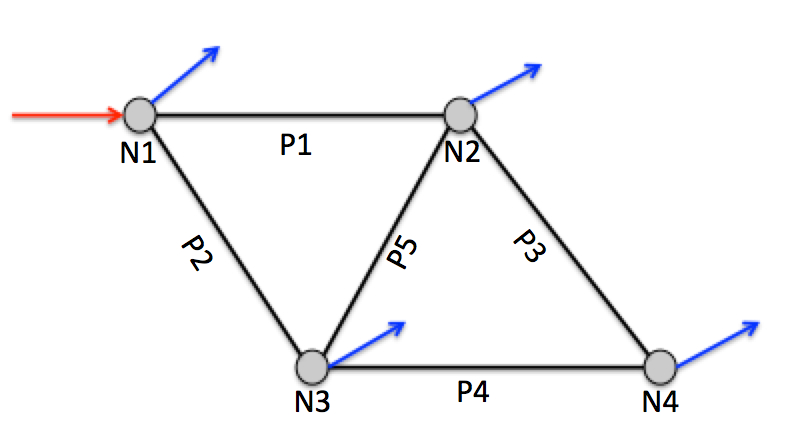
\includegraphics[width=3in]{./8-PipeNetworkHydraulics/NetworkLayout.jpg}
   \caption{Layout of Simple Network}
   \label{fig:NetworkLayout} 
\end{figure}

% Requires the booktabs if the memoir class is not being used
\begin{table}[htbp]
   \centering
   \caption{Node and Pipe Data}
    \begin{tabular}{p{1in} p{1in} p{1in} p{1in} } % Column formatting, @{} suppresses leading/trailing space
    \hline
    \hline
Pipe ID & Diameter (inches) & Length (feet) & Rougnhess (feet) \\
\hline
P1 & 8 & 800 & 0.00001  \\
P2 & 8 & 700 & 0.00001  \\
P3 & 8 & 700 & 0.00001  \\
P4 & 8 & 800 & 0.00001  \\
P5 & 6 & 600 & 0.00001  \\
\hline
\hline
Node ID & Demand (CFS) & Elevation (feet) & Head (feet) \\
\hline
N1 & 2.0 & 0.0 & 100 \\
N2 & 4.0 & 0.0 & ~? \\
N3 & 3.0 & 0.0 & ~? \\
N4 & 1.0 & 0.0 & ~? \\
   \end{tabular}
   \label{tab:PipeData}
\end{table}

Code the script, build an input file, and determine the flow distribution
In your solution you are to supply
\begin{enumerate}
\item An analysis showing the development of the node-arc incidence matrix based on the flow directions in Figure \ref{fig:NetworkLayout},
\item The input file you constructed to provide the simulation values to your script, and
\item A screen capture (or output file) showing the results.
\end{enumerate}


\item Code the script and determine the flow distribution in Figures \ref{fig:pipe-net} and \ref{fig:pipe-net-loops}.  Assume Node N1 has a total head of 300 feet. 

\begin{figure}[h!] %  figure placement: here, top, bottom, or page
   \centering
   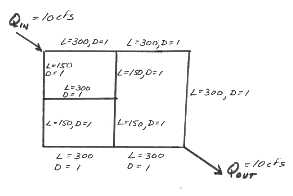
\includegraphics[width=4.5in]{./8-PipeNetworkHydraulics/pipe-net.jpg} 
   \caption{Pipe network for illustrative example with supply and demands identified.  Pipe lengths (in feet) and diameters (in feet) are also depicted.}
   \label{fig:pipe-net}
\end{figure}

\begin{figure}[h!] %  figure placement: here, top, bottom, or page
   \centering
   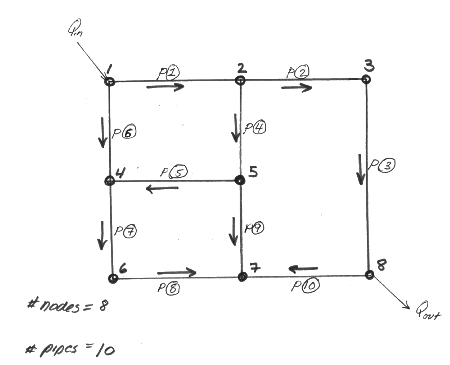
\includegraphics[width=4.5in]{./8-PipeNetworkHydraulics/pipe-net-loops.jpg} 
   \caption{Pipe network for illustrative example with pipes and nodes labeled.}
   \label{fig:pipe-net-loops}
\end{figure}

In your solution you are to supply
\begin{enumerate}
\item An analysis showing the development of the node-arc incidence matrix based on the flow directions in Figure \ref{fig:pipe-net-loops},
\item The input file you constructed to provide the simulation values to your script, and
\item A screen capture (or output file) showing the results.
\end{enumerate}

\item Modify the script to include node elevation information to compute pressures.  Assume all nodes are at elevation 200 feet.
\item (Advanced) Assume the supply Node N1 in the problem in Figure \ref{fig:pipe-net-hybrid} has total head of 100 feet, as shown.  
Assume all the other nodes are at elevation 200 feet.  
Modify the algorithm and script to replace Pipe 1 with a pump with the following pump curve. 
\begin{equation}
h_p = H_{\text{shutoff}} - K_{pump}Q^2
\end{equation}

\end{enumerate}
